\chapter{基于样本的快速图像填充}
 \label{cha:Inpainting}
 本章针对图像填充问题进行了研究,提出了一种基于样本的快速图像填充算法。为了使填充后的图像保持图像原有的结构信息,该算法以由粗到精的方式对图像中的缺失部分进行两次填充。在第一次填充时,首先利用离散小波变换(DWT)对输入图像进行预处理。利用DWT的特点,提取低频子带下的低分辨率图像。利用基于样本的填充方法在此低分辨率图像上进行填充。由于低分辨率图像中的高频细节部分已经被去掉,因此第一遍填充的图像的纹理和大部分结构信息都恢复得不错,但是在包含边界的局部区域还存在着一些瑕疵。为了解决这一问题,对原图像进行第二次填充,在这次填充时只处理包含边缘结构信息的部分,使得这部分区域的结构信息能够与图像的其他部分保持连续性。为了提高图像填充的速度,提出了以动态搜索窗口结合分块结构测试的方式来搜索最佳匹配块。实验结果证明,本章所提的算法能够处理各种困难情况,达到了与目前最好的算法相近的效果。但是,本章所提的算法速度明显优于这些算法。
 \section{研究背景}
 \label{background}
 图像填充问题的主要困难在于使得图像中填充后的区域在内容和结构上与周围区域保持连续性以及算法的效率。相比而言,基于样本的算法在处理结构连续性方面更好。基于样本的算法的出发点是图像中缺失部分的像素,可以以分块为单位,利用图像中已知区域中的一个或多个最佳匹配分块来填充。Criminisi等人~\cite{Criminisi04regionfilling}提出了一种基于未知区域边界法线辐射度方向计算填充优先级算法,使得未知区域以一种类似``剥洋葱皮''的顺序进行填充。虽然该算法在一些缺失部分以纹理区域为主的图像中取得了不错的效果,但是对于缺失部分包含明显图像边缘等结构信息的情况却效果不佳。如图~\ref{fig:criminisi}所示,图~\ref{fig:criminisi:1}是待处理图像,其中黑色区域为缺失部分,图~\ref{fig:criminisi:2}为文献~\inlinecite{Criminisi04regionfilling}中算法的处理结果。可以看出,填充后的三角形金字塔尖并没有恢复,填充结果存在明显的不连续情况。Xu等人~\cite{Xu:2010}指出 为了保持结构部分的连续性,应该优先填充那些包含结构信息的分块。对于图~\ref{fig:criminisi:1}中的未知区域,金字塔部分具有明显的边缘结构信息,而天空部分则为平坦的纹理区域。如果在填充时优先填充金字塔部分然后在填充天空部分,则可以避免用包含金字塔部分的分块去填充天空部分。\par
 \begin{figure}[htb]
   \centering%
   \subcaptionbox{输入图像\label{fig:criminisi:1}} %标题的长度,超过则会换行,如下一个小图。
     {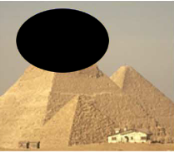
\includegraphics[width=0.3\textwidth]{fillM.png}}%
  \hspace{1em}%
   \subcaptionbox{文献~\inlinecite{Criminisi04regionfilling}算法填充结果\label{fig:criminisi:2}}
       {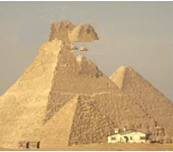
\includegraphics[width=0.3\textwidth]{fillMC.png}}
   \caption{文献~\inlinecite{Criminisi04regionfilling}算法失败例子}
   \label{fig:criminisi}
 \end{figure}
 在基于样本的图像填充算法中,由于像SSD这样的分块相似性度量指标的计算复杂度为$O(N_2)$,且搜索空间为图像全部已知区域,寻找每个缺失部分分块的最佳匹配块是一项非常耗时的工作。对于中等大小的图像,一些算法~\cite{Xu:2010}需要几分钟的时间来处理,这其中大部分时间用于分块的比较和搜索上。在实时或在线图像编辑等实际应用中,用户一般无法忍受超过1分钟的处理时间。\par
 针对以上两方面的问题,本章提出利用基于梯度结构张量(gradient structure tensor,GST)来确定填充顺序,保持填充后图像的结构连续性。为了提高算法速度,提出了一种高效的分块结构测试方法对分块进行结构相似性度量,当分块间的结构信息存在较大差距时可以直接判为不匹配分块,减少冗余的SSD计算。同时,为了减少最佳匹配块的搜索范围,提出了一种动态搜索窗口算法,利用图像的连续性减少搜索范围。在分块匹配时,提出了用加权SSD代替SSD进行,以改进分块间的匹配度。

 \section{算法描述}
 \label{algorithm}
 设输入图像\emph{I} 中包含未知区域 \(\Omega\) 已经已知区域 \(\overline{\Omega}\),本章提出的基于样本的图像填充算法的目标是通过\(\overline{\Omega}\)的信息来计算 \(\Omega\)。和其他经典的基于样本的填充算法那一样,本章所提算法的主要任务是确定填充优先级以及寻找最佳匹配块。
 \subsection{基于GST的填充优先级}
 \label{sec:sub:GST}

 定义未知区域\(\Omega\) 的轮廓为 \(\partial\Omega\), 对于 \(\partial\Omega\)上的每个像素\(p\),将以\(p\)为中心的分块\(\Psi_p\)的填充优先级定义为:
 \begin{equation}
    \label{equ:chap3:order}
    P(p)=C(p)\times D(p)
 \end{equation}

 其中 \(C(p)\) 表示可靠性项\cite{Criminisi04regionfilling},具体定义为: $$C(p)=\frac{\sum_{q\in\Psi_p\bigcap\overline{\Omega}}{C(q)}}{\left\vert{\Psi_p}\right\vert},其中$$\(\left\vert.\right\vert\)  表示计算分块中的像素数. 引入\(C(p)\) 的目的在于让那些包含更多已知像素的区域获得更高的优先级。~\ref{equ:chap3:order}中\(D(p)\) 是数据项,主要评估分块中包含结构信息的情况,增加那些包含较多结构信息分块的填充优先级。Xu等人\cite{Xu:2010}和Lemeur等人\cite{LeMeur_2011}分别提出了不同的\(D(p)\)计算方法。本章中提出了一种基于GST的方法。由于GST可以很好的描述图像的结构信息以及梯度方向,已经被广泛运用于图像处理领域\cite{Kothe03edgeand}。 \par
  对于图像\(I\), 其GST定义为:
  $$T=\left(\begin{array}{cc}T_{11} & T_{12} \\ T_{21} &T_{22}\end{array}\right)=\left(\begin{array}{cc}\overline{I_{\sigma,x}^2} & \overline{I_{\sigma,x}I_{\sigma,y}} \\ \overline{I_{\sigma,x}I_{\sigma,y}} & \overline{I_{\sigma,y}^2}\end{array}\right),$$
  其中 \(I_{\sigma,x}\) and \(I_{\sigma,y}\)  为图像在水平方向和垂直方向上的梯度 ,\(\overline{X}\) 表示高斯核函数\(G_{\hat{\sigma}}\) 与 \(X\)的卷积. \(T\) 的特征值 \(\lambda_1\) 和 \(\lambda_2\) 可以反映图像所包含的结构信息情况。在包含较强边缘信息的区域有 \(\lambda_1>\lambda_2\approx0\) ,而在不含边缘的平坦区域则有\(\lambda_1\approx\lambda_2\approx0\)。 \( \lambda_{1,2} \) 可以通过下式计算: $$\lambda_{1,2}=\frac{1}{2}\left(T_{11}+T_{22}\pm\sqrt{\left(T_{11}-T_{22}\right)^2+4T^2_{12}}\right)$$
  其所包含结构的方向信息可以通过下式计算:
 $$\phi=\frac{1}{2}\arctan{\left(\frac{2T_{12}}{T_{11}-T_{22}}\right)}$$
 为了评估每个分块中是否包含结构信息已经结构的方向信息,LeMeur
 等人\cite{LeMeur_2011}提出计算分块中心点的GST。为了得到区域内更为准确的结构信息,本章算法提出计算分块内所有已知像素的GST,并对结果进行直方图统计。该直方图 \(H\) 以分块内包含的结构方向作为直方图分块依据,统计区域内已知像素的结构能量 \(\lambda_1\)。相比于文献\cite{LeMeur_2011}的方法,本章算法得到的是整个分块的结构信息,比文献\cite{LeMeur_2011}只计算分块中心点的GST的方法更鲁棒。在本章算法中\(H\)的大小(直方图中Bin的数量)为12。定义分块结构能量(patch structure energe, PSE):
 $$P_e\left(p\right)=Max\left(Sum_{b\in{H\left(p\right)}}\left(b\right)\right)$$, 其中\(H\left(p\right)\) 表示结构能量直方图。 对于图像\(I\) , 公式~\ref{equ:chap3:order}中的数据项定义为:
 $$D(p)=(1-\alpha)P_e(p)/max_{q\in{I}}(P_e(q))+\alpha,$$ 其中 \(\alpha\) 是一个线性变换因子,使得\(D(p)\in{[\alpha,1]}\)。加入\(\alpha\) 的目的是使得数据项的值接近于可靠性项值。在本章算法中,参考文献\cite{Xu:2010}的建议,将\(\alpha\)设为固定值0.2。
 \subsection{加权SSD}
 \label{sec:sub:WSSD}
 为了寻找样本分块\(\Psi_p\)的最佳匹配块,Criminisi等人\cite{Criminisi04regionfilling}借助于两个分块间已知像素的SSD类评估分块间的相似性。待填充分块\(\Psi_p\)的最佳匹配块定义为
 \begin{equation}
 \label{equ:cha03:bestmatch}
 \Psi_{\hat{q}}=arg\;min_{\Psi_q\in\Phi}d(K\Psi_p,K\Psi_q)
 \end{equation}
 其中,\(d(.,.)\) 表示计算两个分块之间的 SSD , \(K\) , \(\Phi\)表示搜索范围。实际上,仅仅依靠分块已知区域的SSD是无法保证找到的最佳匹配快都是最合适用于填充的分块。例如,如图~\ref{cha03:fig:1}所示,蓝色的分块为待填充分块,绿色分块为用公式~\ref{equ:cha03:bestmatch}计算得到的最佳匹配块。从图中可以看到,在一些情况下仅靠分块已知区域的SSD不能找到合适的填充块。
 \begin{figure}[!htbp]
 	\begin{center}
 			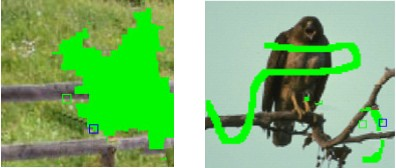
\includegraphics[width=0.8\columnwidth]{ch3/fig1.jpg}
 	\end{center}
     \caption{使用已知分块内SSD搜索造成错误匹配情况}
 	\label{cha03:fig:1}
 \end{figure}
 在文献 \inlinecite{kwokFast}中,提出了一种基于梯度的预填充方法,对待填充分块内的未知像素进行估计。基于同样的预处理方法,。文献\inlinecite{jemi:2011}提出使用已知和未知区域的加权SSD (Weighted SSD,WSSD)来寻找最佳匹配块。该算法的预填充算法假设未知区域内的像素梯度值为零。基于这一假设,未知区域的像素颜色值可以通过梯度方程的最小二乘法来求解。然而,实际应用中图像较难满足梯度值为零这一假设。这这种预处理方法只考虑了分块内的局部梯度信息,最终的预处理结果并不明显。 Xu等人\cite{Xu:2010}指出,待填充分块内新填充的像素应该与周围分块保持颜色一致性和连续性。基于这一思路,本章提出了一种新的预处理方法。
 为了方便比较,本章中使用与文献\inlinecite{Xu:2010}一致的符合标识。假设 \(N(p)\) 为中心点在\(p\)的邻域窗口,集合\(N_s(p)\)定义为:
 $$N_s(p)= \left\{ p_j:p_j \in N(p)\;and\;\Psi_{p_j} \subset \overline{\Omega} \right\}.$$
 分块 \(\Psi_p\) 和\(\Psi_{p_j}\)  之间的相似性定义为:
 $$\omega_{p,p_{j}}=\frac{1}{Z(p)}exp\left(-\frac{d(K\Psi_p,K\Psi_{p_j})}{\sigma^2\left|K\Psi_p\right|}\right)$$
 其中 \(Z(p)\) 为归一化因子使得 $$\sum_{p_j\in N_s(p)}\omega_{p,p_j} = 1$$ , \(\sigma\) 为固定值5.0 \cite{Xu:2010}.\par
 令运算符\(U\) 表示从分块中提取未知像素,分块 \(\Psi_p\) 中的未知像素的预填充为
 $$U(p)=U\left(\sum_{p_j \in N_s(p)}{\omega_{p,p_j}\Psi_{p_j}}\right)$$\par
 为了寻找待填充分块的最佳匹配块, 本章提出以WSSD的方式来评估分块之间的相似性:
 \begin{equation}
 W(\Psi_p,\Psi_{p_j})=\beta\times d(K\Psi_p,K\Psi_{p_j})+(1-\beta)\times d(U\Psi_p,U\Psi_{p_j})
 \label{chap03:equ:wssd}
 \end{equation}
 其中加权系数 \(\beta\) 为已知区域的权值,从~\ref{chap03:equ:wssd}中可看出WSSD综合考虑了分块未知区域和已知区域的信息。由于未知区域是通过预填充算法估算的,因此加权系数\(\beta\)的值应该大约0.5,让已知部分的权值更大。在本章算法中 \(\beta\)的值建议范围为$[0.8, 0.9]$。综上所述,分块\(\Psi_p\) 的最佳匹配块定义为:


 $$\Psi_{\hat{p}}=arg\;min_{\Psi_q \in \Phi}{W(\Psi_p,\Psi_q)}.$$


 \subsection{最佳匹配块搜索策略}
 在基于样本的图像填充算法中,主要的计算量集中在最佳匹配块的搜索中。为了提高搜索速度,文献\cite{kwokFast}提出了一种基于$K$D-tree的近似最相近邻域搜索算法,该方法主要利用高效的$K$D-tree数据结构对搜索进行加速。本章算法中,以让搜索更智能和更快为目标,提出一种智能搜索策略。由于SSD计算需要对分块每个像素进行比较,效率很低。实际上,我们人眼在搜索匹配块时并不会这样逐个像素去比较。只有当两个分块在外观上十分接近时,才可能进行这样逐个像素的比较。假如要人工完成最佳匹配块的搜索工作,人们会首先将那些明显不一致的分块放到一边不予考虑。这个预先判断和筛选的过程非常重要,本章提出利用分块结构测试的方式对分块进行测试,判断分块间结构信息是否一致。对于那些在结构上明显不一致的分块,可以直接将其排除在外,减少冗余的计算,从而加快搜索的速度。
 \subsubsection{分块结构距离测试}
 \label{sec:sub:PST}
 在~\ref{sec:sub:GST}中,分块GST直方图被用于描述分块的结构信息。对于相似的分块,他们之间的SSD会相对较小,因此他们一定包含相似的结构信息。例如,同为不包含结构信息的两块纹理信息为主的分块,或者同为包含垂直方向边缘结构信息的分块等。对于这些相似的分块,他们的分块直方图分布也会比较相似。假如两个分块\(\Psi_p\) 、\(\Psi_q\)的GST直方图分别为 \(H(p)\) 和 \(H(q)\),本章算法将他们之间的分块结构距离(patch structure distance, PSD)定义为\(H(p)\) 和\(H(q)\)之间的相关系数,即:

 $$PSD(p,q)=\frac{\acute{\sigma}_{pq}+c}{\acute{\sigma_p}\acute{\sigma_q}+c},$$
其中\(\acute{\sigma}_{pq}\) 为 \(H(p)\)与 \(H(q)\)之间的协方差, \(\acute{\sigma_p}\) 及 \(\acute{\sigma_q}\) 分别为 \(H(p)\) 与\(H(q)\)的标准差, \(c\) 是一个很小的常数避免出现零除以零的情况。\par
 对于待填充分块 \(p\)以及搜索窗口内的分块\(q\),当\(PSD(p,q)\)大于某门限,本章算法中门限值设置为(0.5\(\sim\)0.6, 那么认为\(p\) 和 \(q\)在结构上存在较大差异,这也就意味着\(q\) 不可能是要寻找的最佳匹配块。这时也就没有必要再去计算他们之间的SSD。 基于此,对于候选分块\(c\),在计算 \(p\) 与 \(c\)之间的SSD时,首先测试这两者之间的PSD值是否在可接受的范围之内。对于通过PSD测试的分块,再通过SSD进一步评估分块之间的相似性,而PSD测试没有通过的分块可以直接忽略。由于\(\overline{\Omega}\)范围内所有分块的分块GST直方图可以预先计算,且PSD的计算复杂度远低于SSD, 引入PSD测试可以节省很多SSD的冗余计算。\par
例如,在图~\ref{chap03:fig:PSD}中, 蓝色的分块为待填充分块,绿色矩形之内为最佳匹配块搜索范围, 红色分块为通过PSD测试的候选分块,黑色分块为本章算法搜索到的最佳匹配。从图~\ref{chap03:fig:PSD}中可以看到,由于蓝色的待填充分块包含垂直方向的边缘,所有包含水平方向边缘的分块均没有通过PSD测试。因此这些分块不可能是最佳匹配分块目标,可以直接忽略。
 \begin{figure}[!htbp]
 	\begin{center}
 			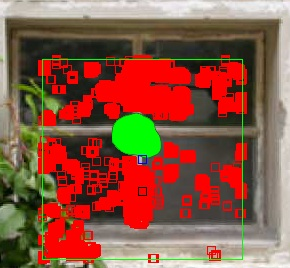
\includegraphics[width=0.6\columnwidth]{ch3/fig2.jpg}
 	\end{center}
     \caption{PSD测试示意图}
 	\label{chap03:fig:PSD}
 \end{figure}


 \subsection{动态搜索窗口}
 \label{sec:sub:dynamicSearch}
 在传统的基于样本的图像填充算法中,公式~\ref{equ:cha03:bestmatch}中的 \(\Phi\)为以每个待填充区域为中心的固定窗口\cite{LeMeur_2011},或者是全部未知区域\inlinecite{Criminisi04regionfilling}。 设 \(\Psi_p\) 为中心在\(p\)处的待填充分块,考虑到图像局部范围的连续性,在\(p\)附件找到\(p\)的最佳匹配块的概率应该较大。因此定义局部窗口
 $$Win_l(p)=Win(p,sizeL)\cap \Omega,$$
 其中 \(Win(p,sizeL)\) 是大小为 \(sizeL\times sizeL\)中心点在 \( p\)的矩形窗口. \par
 收到快速近似最相似邻域搜索算法PatchMatch \cite{Barnes:2009}的启发,利用图像的连续性特点,本章提出了利用邻域窗来提高搜索效率。假设 \(\Psi_q\)为 \(\Psi_p\)的相邻分块 ,即\(p\) 与\(q\)之间的距离与分块大小相等。如果 \(\Psi_q\) 已经完成了填充 ,且其最佳匹配快为 \(\hat{q}\)。那么根据图像的连续性特点,  相邻分块\(\Psi_p\)的最佳匹配块与 \(\hat{q}\)相邻的概率也会较大。 因此,定义邻域搜索窗口如下:
 $$Win_n(p)=Win(\hat{q},sizeN)\cap\Omega.$$ 
 当\(p\)的相邻分块中还没有一个完成填充时,\( Win_n(p)=\emptyset  \)。结合局部窗口全部搜索区域定义为:
 $$\Phi=Win_n(p)\cup Win_l(p).$$
 在图\ref{ch3:fig:3}中展示了搜索范围的一个例子。图\ref{ch3:fig:3}中,蓝色的分块为待填充分块,邻域搜索窗口和局部搜索窗口分别用红色和绿色标识,搜索到的最佳匹配块用黑色标识 。通过这种搜索方式,在图像填充过程中每个分块的最佳匹配块可以在更小的动态范围内被搜索到。因为邻域窗口的引入,局部窗口的大小可以设置得更小。在本章算法中,局部窗口和邻域窗口分别被设置为8\(\sim\)10 以及5\(\sim\)7 倍的分块大小。对于那些邻域窗口为零的分块,可以增大其局部搜索窗口的大小。\par
 \begin{figure}[!htbp]
 	\begin{center}
 			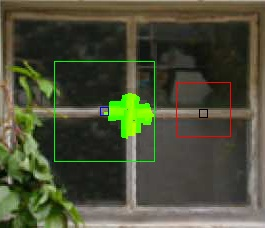
\includegraphics[width=0.6\columnwidth]{ch3/fig3.jpg}
 	\end{center}
     \caption{局部搜索窗口与邻域搜索窗口}
 	\label{ch3:fig:3}
 \end{figure}
 综上所述,本章提出的改进的基于样本的图像填充算法见\ref{ch3:alg:inpainting}。
 \renewcommand{\algorithmcfname}{算法}
\begin{algorithm}[!htb]
\LinesNumbered
\KwData { 图像 \(I\),其中未知区域 \(\Omega \) ,已知区域 \(\overline{\Omega}\),  \(\Omega \) 的轮廓为 \(\partial \Omega\)}
\KwResult {填充后的图像}

   \ForEach {分块 $\Psi_q \in \overline{\Omega}$ }{
   计算分块能量直方图\(H(q)\)\;}
   
   \ForEach { \(\partial \Omega\)上的像素 \(p\) }{
   	 计算以$p$为中心的分块\(\Psi_p\)\ 的结构能量直方图以及PSE\;
   	 计算\(\Psi_p\) 的填充优先级 $Pri[\Psi_p]$\;}
   \While{\( \Omega \neq null\) }{
	$\Psi = \arg max_{p \in \partial \Omega}Pri[p]$\;
    按照 \ref{sec:sub:dynamicSearch} 中的方法计算搜索窗口\(\Phi\) \;
    \ForEach {$\Psi_q$ in \(\Phi\)}{ 
    $d = PSD( \Psi_q,\Psi)$\;
     	\If{d < threshold}  
     		{利用公式\ref{chap03:equ:wssd}计算$wd[\Psi_q]=WSSD(\Psi_q,\Psi)$\;}
     	 
     	 \Else
     	 	{ $wd[\Psi_q]=MAX$\;}
     $\Psi_m = \arg min_{p \in \phi }wd[p]$ \;
     利用 \(\Psi_m\)的对应像素填充 \(\Psi\) 中的缺失部分\;
     更新\(\partial \Omega\)\;
     \ForEach{\(\partial \Omega\) 上新增像素\(n\) }
     {
     计算 \(\Psi_n\)的填充优先级$Pri[\Psi_n]$\;
     }
   }
   }
\label{ch3:alg:inpainting}
\caption{基于样本的图像填充}
\end{algorithm}
 
\subsection{两阶段由粗到精图像填充}
\label{sec:2.2}
对于图像填充算法来说,主要的困难在于保持输入图像中连续的结构和纹理信息以及尽可能减少图像填充过程的运算量。为了加快算法的速度,首先对输入图像进行预处理,降低其分辨率。 对输入图像进行DWT,选取低频子带图像作为输入图像的低分辨率版本。由于DWT的低频部分可以保留图像中的结构信息,因此在此低分辨率版本图像上进行填充可以保持原图中的结构信息。并且,由于低分辨率图像大小是原图像的四分之一, 使得填充速度是原图像的四倍。\par
在文献\inlinecite{LeMeur:2012}中,提出了一种与本章算法类似的两阶段填充算法,不同之处是文献\inlinecite{LeMeur:2012}算法使用超分辨率算法从填充后低分辨图像中恢复到原图像分辨率。虽然低分辨率下填充算法可以更快,但是由于随后的超分辨率算法耗时远大于填充算法那,造成整个算法并没有加快速度 。与文献\inlinecite{LeMeur:2012}不同,本章算法中输入图像可以与低分辨率图像同时填充。例如,在图~\ref{ch3:fig:4}中,左边的图像\(C\)为输入图像的低分辨率版本,右边图像为相应的输入图像\(O\); 假如分块 \(\Psi_c\) in \(C\) located at \((x,y)\), its best-match patch \(\Psi_{\hat{c}}\) is found to be located at \((i, j)\), then the corresponding patch \(\Psi_o\) in \(O\) located at \((2x, 2y)\) can be inpainted via the corresponding match patch \(\Psi_{\hat{o}}\) located at \((2i, 2j)\).
\begin{figure}[!htbp]
	\begin{center}
			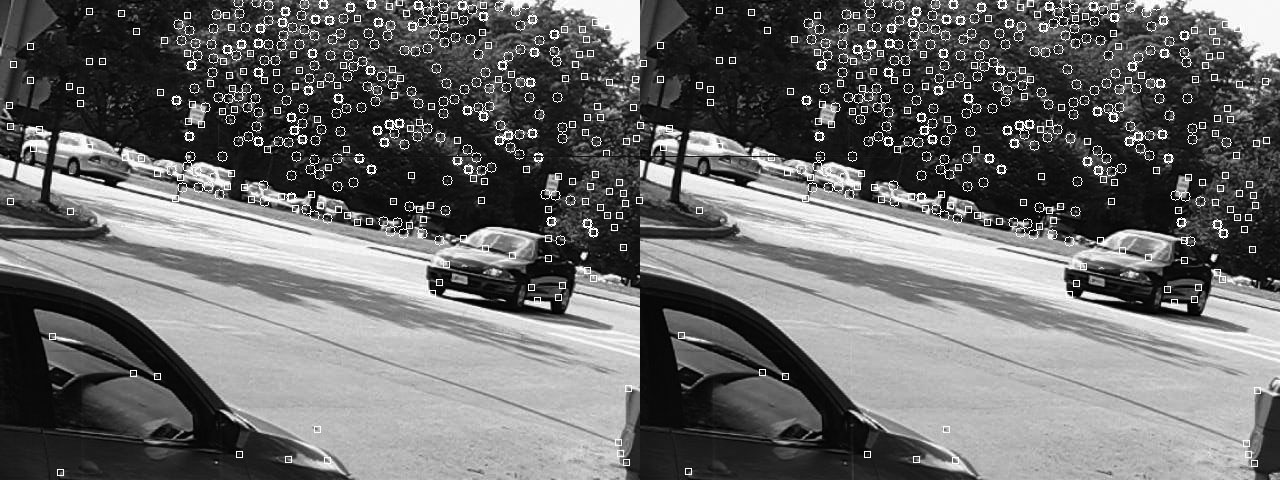
\includegraphics[width=0.8\columnwidth]{ch3/fig4.jpg}
	\end{center}
    \caption{Image inpainting based on the coarse-version image}
	\label{ch3:fig:4}
\end{figure}
The flow chart of the proposed two-step inpainting algorithm is shown in Fig.5. In the first inpainting, both the coarse-version and the original input image can be inpainted synchronously, but only the inpainting result at original resolution is required for the following step.\par
% For one-column wide figures use
\begin{figure}[!htbp]
\begin{center}
% Use the relevant command to insert your figure file.
% For example, with the graphicx package use
  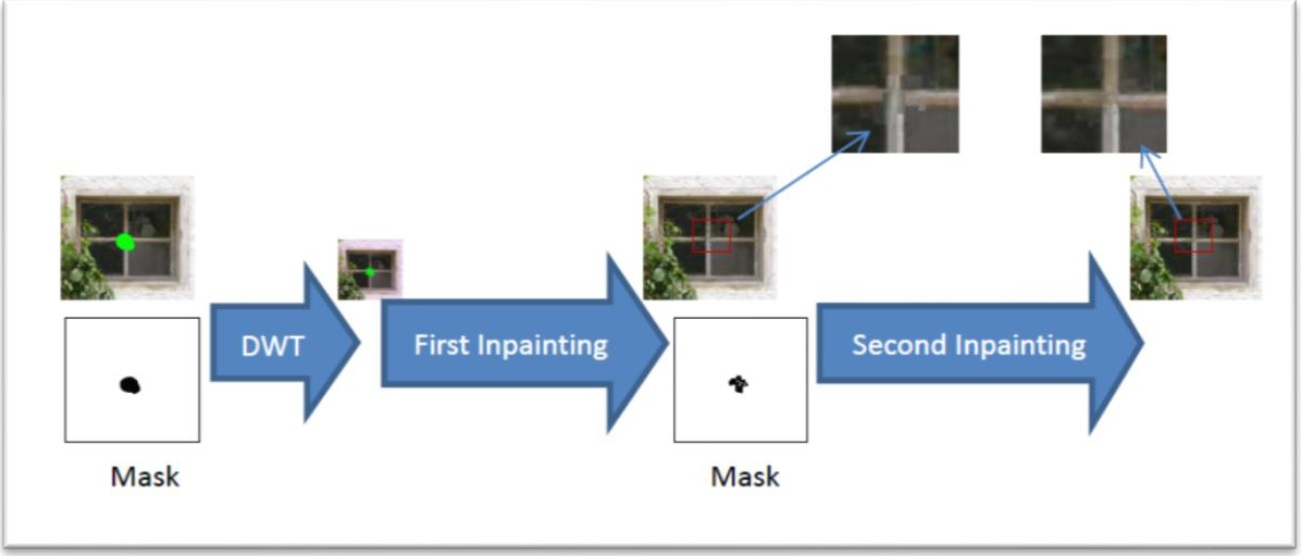
\includegraphics[width=0.5\textwidth]{ch3/fig5.jpg}
% figure caption is below the figure
\end{center}
\caption{Flow chart of two-step inpainting}
\label{fig:5}       % Give a unique label
\end{figure}
We can see that the first-time inpainted image(shown in the middle of Fig.5) can recover most of the structures and textures, but some artifacts exist in the edge regions (marked by the red rectangle with a zoomed-in version shown in the right-top). To overcome this defect, the second inpainting is performed only in these areas. The edge regions with artifacts can be located through PSE. The pixels that need to be inpainted twice are defined as \(\forall p \in \Omega, P_e(p)>E_{Thres}\). In this paper, \(E_{Thres}\) is set to \(0.015*Max_{q\in{I}}{(P_e(p)})\). In the middle of Fig.5, we can see that the updated mask for the second inpainting is smaller than the original one, and only covers those areas with artifacts. In the first inpainting, the missing regions are firstly estimated by the prefill method, then the output of the first inpainting will be used as the input of the second inpainting. In the second inpainting, the missing regions are already been estimated by the first inpainting, so the prefilling process can be omitted.
 


 \section{实验结果与分析}
 \label{cha3:results}
Our algorithm is tested on a variety of natural images. In Fig.6, some of the results are demonstrated and compared with the existing state-of-the-art approaches \cite{Criminisi04regionfilling}, \cite{Xu:2010}. In the following examples, the patch size is set to \(7\times7\) in the coarse-version images and \(9\times9\) in the original ones. The size of \(N_s(p)\) is set to 51 as in [3]. The algorithm is implemented with C++ programming language. All the experiments are run on a PC equipped with an Intel 2.67 GHz CPU.\par
\begin{figure*}[!htbp]
\begin{center}
% Use the relevant command to insert your figure file.
% For example, with the graphicx package use
  \includegraphics[width=0.8\textwidth]{ch3/fig6f.jpg}\\
  (a) Mask\quad\quad\quad\quad\quad\quad(b) Criminisi\cite{Criminisi04regionfilling}\quad\quad\quad\quad\quad\quad(c) Xu\cite{Xu:2010}\quad\quad\quad\quad\quad\quad(d) Proposed
% figure caption is below the figure
\end{center}
\caption{Inpainted results and comparison with Criminisi\cite{Criminisi04regionfilling} and Xu\cite{Xu:2010}}
\label{fig:6}       % Give a unique label
\end{figure*}
In Fig. 6, we can see that in the images inpainted by our method, the missing regions can be effectively filled with continuous structures and textures. Our results outperform those inpainted by \cite{Criminisi04regionfilling}, and are close to the results in \cite{Xu:2010}. In our implementation of \cite{Criminisi04regionfilling}'s method, the patch size is set to \(9\times9\), some results are different from those given in \cite{Xu:2010}. The comparison of the computation time is shown in Tab.1, where the images are corresponding to those of Fig.6 from top to down. Because of the lower computational complexity, our algorithm is much faster than both \cite{Criminisi04regionfilling} and \cite{Xu:2010}, thanks to the multi-resolution two-step inpainting, the dynamic search window and PSD test speed up the schemes.
\begin{table}[!htbp]
% table caption is above the table
\caption{Comparison of computation time}
\label{tab:1}       % Give a unique label
% For LaTeX tables use
\begin{tabular}{lllll} \hline
\multicolumn{1}{c}{\multirow {2}{*}{Image}}&\multicolumn{1}{c}{\multirow {2}{*}{Unknown Pixels}}& \multicolumn{3}{c}{Computation time(unit: second)}\\
\cline{3-5}
\multicolumn{1}{c}{}&\multicolumn{1}{c}{}& \multicolumn{1}{c}{Criminisi[2]} &Xu[3]&Proposed\\
\hline
\multicolumn{1}{c}{Pyramid} & \multicolumn{1}{c}{19636} & \multicolumn{1}{c}{83} &\multicolumn{1}{c}{143}& \multicolumn{1}{c}{9}\\				
\multicolumn{1}{c}{Plane} & \multicolumn{1}{c}{17914} & \multicolumn{1}{c}{82} &\multicolumn{1}{c}{130}& \multicolumn{1}{c}{10}\\				
\multicolumn{1}{c}{Riding} & \multicolumn{1}{c}{23161} & \multicolumn{1}{c}{121} &\multicolumn{1}{c}{165}& \multicolumn{1}{c}{25}\\
\multicolumn{1}{c}{Eagle} & \multicolumn{1}{c}{14837} & \multicolumn{1}{c}{84} &\multicolumn{1}{c}{108}& \multicolumn{1}{c}{17}\\
\multicolumn{1}{c}{Beach} & \multicolumn{1}{c}{6281} & \multicolumn{1}{c}{17} &\multicolumn{1}{c}{45}& \multicolumn{1}{c}{4}\\
\hline
\end{tabular}
\end{table}\par

\begin{figure}[!htbp]
\begin{center}
% Use the relevant command to insert your figure file.
% For example, with the graphicx package use
  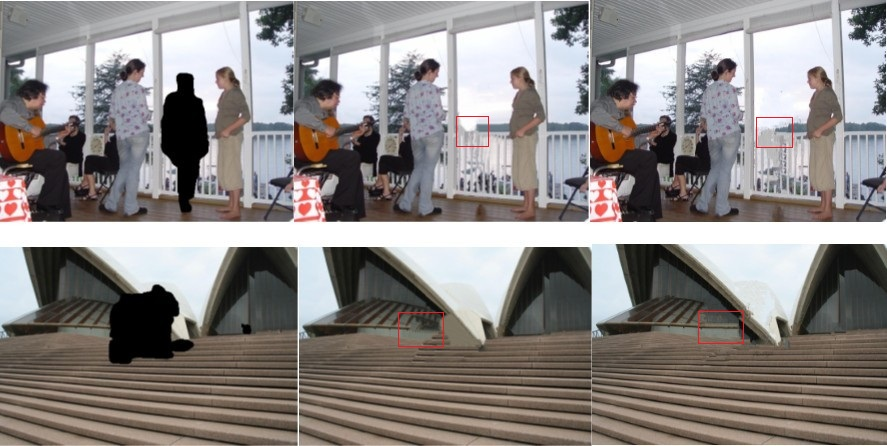
\includegraphics[width=0.5\textwidth]{ch3/fig7.jpg}
% figure caption is below the figure
\end{center}
\caption{Comparision of proposed method with \cite{LeMeur_2011}, left:mask, middle:inpainted by\cite{LeMeur_2011}, right:inpainted by proposed method}
\label{fig:7}       % Give a unique label
\end{figure}

\begin{figure}[!htbp]
\begin{center}
% Use the relevant command to insert your figure file.
% For example, with the graphicx package use
  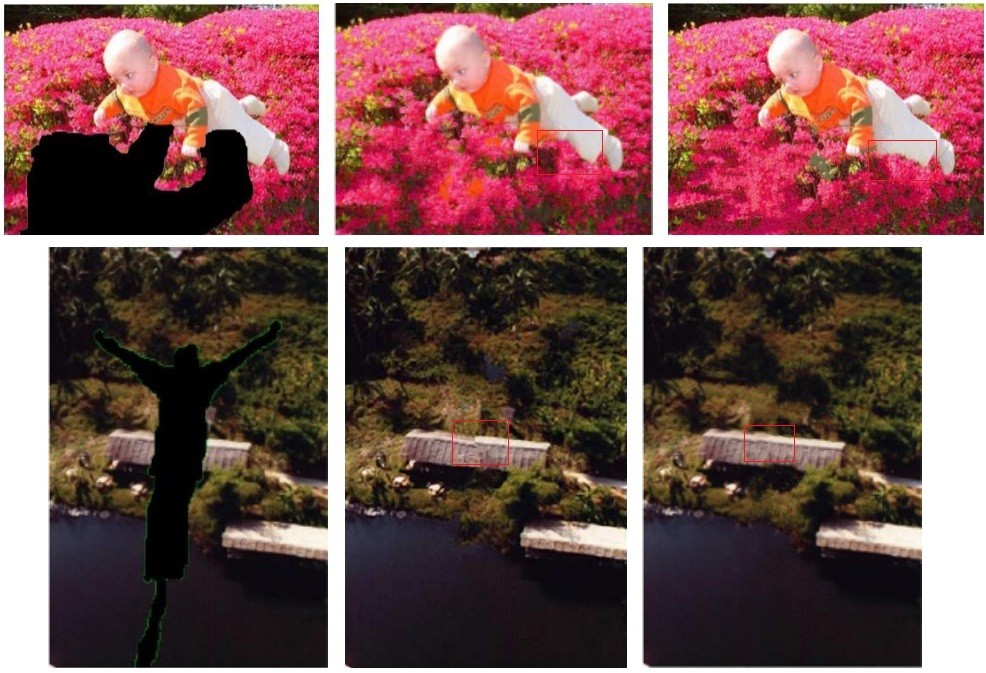
\includegraphics[width=0.5\textwidth]{ch3/fig8.jpg}
% figure caption is below the figure
\end{center}
\caption{Comparision of proposed method with \cite{kwokFast}, left:mask, middle:inpainted by\cite{kwokFast}, right:inpainted by proposed method}
\label{fig:8}       % Give a unique label
\end{figure}

\begin{figure}[!htbp]
\begin{center}
% Use the relevant command to insert your figure file.
% For example, with the graphicx package use
  \includegraphics[width=0.5\textwidth]{ch3/fig9.jpg}
% figure caption is below the figure
\end{center}
\caption{Comparision of proposed method with \cite{LeMeur:2012}, left:mask, middle:inpainted by\cite{LeMeur:2012}, right:inpainted by proposed method}
\label{fig:9}       % Give a unique label
\end{figure}\par
Some other tough examples in \cite{LeMeur_2011}, \cite{kwokFast} and \cite{LeMeur:2012} are also tested with the proposed algorithm. The inpainting results are shown in Figs. 7, 8 and 9 respectively. As illustrated in these figures, the sharp and obvious edges can be well preserved in the inpainted images. This is because the GST-based filling order favours those patches with strong structures. From Figs. 8 and 9, we can see that the proposed method sometimes produces repeated texture patterns, especially in images mainly with textures. This is caused by the neighbor window introduced in the best-match searching process.

 \section{本章小结}
 \label{cha3:conclusions}
In this paper, a fast two-step examplar-based image inpainting algorithm is presented. The first inpainting is based on the coarse version of the input image, in which the high-frequency details are filtered by DWT. Then the second inpainting is performed only in the areas that contain edges at the original resolution. In the second inpaiting, results of first inpainting are treated as prefill result, and are computed as a part of the \(WSSD\), in such a way that the structural information of the known regions of the input image can be well propagate into the missing regions. The main merits of this algorithm are in the following four points:\begin{itemize}
                                \item first, the DWT based two-step inpainting scheme can quickly obtain the inpainted results at the original resolution;
                                \item second, the GST based filling order enables sharp structures to be preserved in the inpainted result;
                                \item third, the prefilling scheme based on the image locality and continuity is more effective and accurate;
                                \item forth, using the dynamic search window and PSD test, the best-match searching process can be smarter and faster.
                              \end{itemize}
Compared with the state-of-the-art algorithms, our method is simpler and easier to implement, and the results are comparable, but the computation cost is much lower. In some applications, real-time image inpainting is required and can be done via parallelization and GPU computing \cite{kwokFast}. We will consider this in the future work.